%%%%%%%%%%%%%%%%%%%%%%%%%%%%%%%%%%%%%%%%%%%%%%%%%%%%%%%%%%%%%%%%%%%%%%%%%%%%%%%
%%%%%%%%%%%%%%%%%%%%%%%%%%%%%%%%%%%%%%%%%%%%%%%%%%%%%%%%%%%%%%%%%%%%%%%%%%%%%%%
%%%%%%%%%%%%%%%%%%%%%%%%%%%%%%%%%%%%%%%%%%%%%%%%%%%%%%%%%%%%%%%%%%%%%%%%%%%%%%%
%%%%%%%%%%%%%%%%%%%%%%%%%%%%%%%%%%%%%%%%%%%%%%%%%%%%%%%%%%%%%%%%%%%%%%%%%%%%%%%
\section{The Experimental Setup and Dataset}
%%%%%%%%%%%%%%%%%%%%%%%%%%%%%%%%%%%%%%%%%%%%%%%%%%%%%%%%%%%%%%%%%%%%%%%%%%%%%%%
%%%%%%%%%%%%%%%%%%%%%%%%%%%%%%%%%%%%%%%%%%%%%%%%%%%%%%%%%%%%%%%%%%%%%%%%%%%%%%%
%%%%%%%%%%%%%%%%%%%%%%%%%%%%%%%%%%%%%%%%%%%%%%%%%%%%%%%%%%%%%%%%%%%%%%%%%%%%%%%
%%%%%%%%%%%%%%%%%%%%%%%%%%%%%%%%%%%%%%%%%%%%%%%%%%%%%%%%%%%%%%%%%%%%%%%%%%%%%%%

The dataset is derived from high-resolution video files that capture tagged honey bees of one colony in a single frame observation hive.
The bees are uniquely tagged with circular 12-bit markers (Figure~\ref{fig:markers}, section~\ref{ch:intro}).
Two cameras per side filmed the complete honeycomb.
Figure~\ref{fig:obssetup} illustrates the camera setup.
The \emph{recording period} lasted nine weeks (63 days), from July~19,~2016 until September~19,~2016, with some interruptions due to maintenance work and technical failures.
An overview about the complete recording period is given in Figure~\ref{fig:observation-period}.

\begin{figure}[htbp]
	\centering
	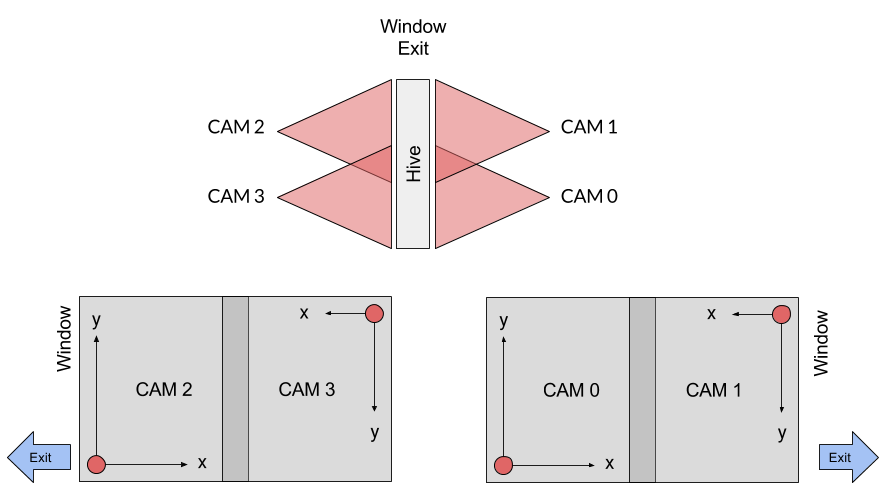
\includegraphics[width=1.0\textwidth]{Figures/setupCams}
 	\caption[Observation setup]{\textbf{Observation setup} Each side of the honeycomb is filmed by two cameras. The two cameras per side overlap, so bees inside this area are detected from both cameras.}
 	\label{fig:obssetup}
\end{figure}

All four cameras, each with a resolution of $4000\times3000$ pixel, recorded $3.5$ frames per second. 
An image analysis pipeline~\cite{wario2015automatic} detects all bees in each frame.
The resulting detection data is stored in a binary file format.
A python library\footnote{The library is called bb-binary and is created by the Biorobotics Lab. It can be found on GitHub: \url{https://github.com/BioroboticsLab/bb_binary}; Last accessed: February 16, 2016; 4:28~p.m.} provides a frame-level access to those binary files.
The size of the dataset is $470$~GB, about $7.5$~GB of binary data per day.

The 67 day \emph{tagging period} began on June~28,~2016 and lasted until September~2,~2016, resulting in 3,191 tagged bees.
Bees were already tagged three weeks before the observation started.
The young bees, which were raised in a separate incubator, were tagged and then added to the observation hive at noon each day.
Figure~\ref{fig:tagging-period} shows the frequency of tagged bees per day.
The hatching day for each bee is documented and therefore the age of each bee at a particular point in time can be calculated.
The life expectancy of a honey bee during summer ranges from 30 to 60 days, according to \textcite[p.~27]{menzel2016intelligenz}
The maximum number of present bees in the hive is about 1,600.